
\usetikzlibrary{automata, positioning, arrows}

\begin{document}
	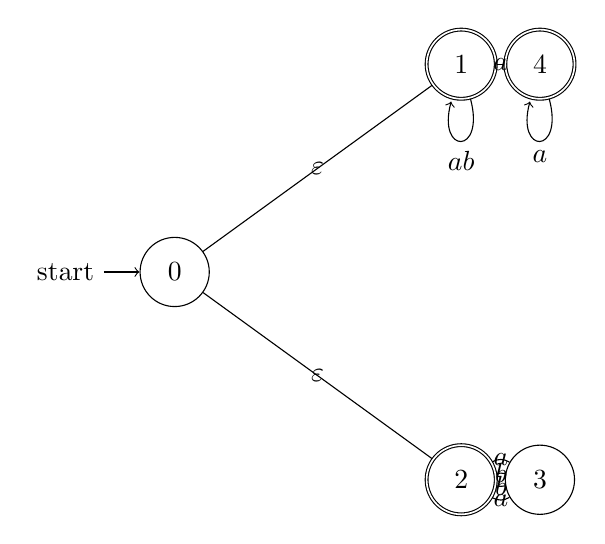
\begin{tikzpicture}
		\node [state, initial] (0) {0};
		\node [state, accepting, above right = 2cm and 3cm of 0] (1) {1};
		\node [state, accepting, below right = 2cm and 3cm of 0] (2) {2};
		\node [state, right of = 2] (3) {3};
		\node [state, accepting, right of = 1] (4) {4};

		\path
		(0) edge node {$\varepsilon$} (1)
		edge node {$\varepsilon$} (2)
		(2) edge [bend left = 30] node {$a$} (3)
		edge [bend left = 10] node {$b$} (3)
		(3) edge [bend left = 30] node {$a$} (2)
		edge [bend left = 10] node {$b$} (2)
		(1) edge [loop below] node {$ab$} (1)
		edge node {$a$} (4)
		(4) edge [loop below] node {$a$} (4);

	\end{tikzpicture}
\end{document}
